%************************************************
\section*{Methodology}\label{ch:methodology}
%************************************************

\subsection*{Research Questions}\label{sec:research_questions}

\textbf{RQ1: What are the characteristics of structural commit-feature interactions?}

We intend to research two main properties which will already provide a lot of insight into the development process of features and usage of commits therein.
Firstly, we will examine the statistical distribution of how many commits, features interact with structurally.
This will directly give an estimation on how many commits were used to create a feature.
Our analysis also allows us to gauge feature-size, which can put the amount of commits used to implement a feature into perspective.
Secondly, we want to examine how many features a commit interacts with structurally, e.g. how many features a commit usually changes. 
This is especially interesting when considering best practices surrounding the usage of commits.
It is preferred to keep commits granular meaning they should only fix a single bug or, in our case, change a single feature.
Acquiring data on this issue will show how strictly this policy is enforced in the development of features. \\

\begin{center}
\begin{tabular}{cc}
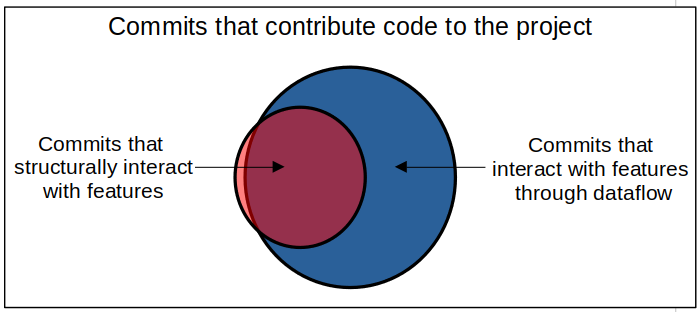
\includegraphics[height=6cm]{gfx/Commits-of-a-Software-Project.png}
\end{tabular}
\captionof{figure}{Kinds of Commits in a Software Project investigated in this work}
\end{center}

\textbf{RQ2: How do commits interact with features through dataflow?}

Previous research has focused solely on dataflow interactions between commits.
We have already discussed the importance of research in the area and why further research is necessary.
That's why we want to provide first insights on the properties of dataflow-based commit-feature interactions.
Specifically, we will investigate how connected commits and features are by analyzing the amount of features a commit usually affects through dataflow.
Knowing what fraction of all commits contributing code to a project are part of dataflow-based interactions will show how often new commits affect the data of a feature. 
Regarding this, it is worth considering that commits constituting code of a feature are very likely to influence the data of said feature.
Since these datflow interactions are so obvious, programmers are also much more aware of them. 
Depending on the prevalence of feature-regions in a project's code space this could heavily skew the data in one direction. 
Therefore we want to especially focus on commits that aren't part of a feature, which will give us more valuable and insightful information. \\

\textbf{RQ3: How do authors implement features?}

Usually there are many programmers working on the same software project, implementing different features, sometimes alone, sometimes with the help of colleagues.
We want to shine some light on the exact statistics of this by combining structural commit-feature interactions with high-level repository information.
One major question we want to answer is how many authors implement a feature on average, where considering feature-size could help put this data into perspective.
Additionally we aim to gauge the amount of code each developer of a feature contributes. 
This way we can recognize development patterns like the existence of a main developer as discussed by \citet{sattler2023seal}. 
The collected results could serve as advice for software companies on how to allocate programmers on to-be implemented features. 

\subsection*{Operationalization}\label{sec:operationalization}

\textbf{RQ1: What are the characteristics of structural commit-feature interactions?}

The needed data will be collected by creating reports comprimising all structural commit-feature interactions of a chosen software project.
The collected data is then evaluated by iterating over all found commit-feature interactions.
For each encountered feature we save the commits it interacts with.
As the analysis has also calculated the amount of instructions a structural interaction occurs in 
we save the entire amount of such instructions for every feature.
We have previously noted that a feature only structurally interacts with a commit that has contributed code to said feature.
Besides that each line of code in a git project was added or changed by a commit, 
which means that each line of code that belongs to a feature also belongs to a commit.
Therefore the commits saved inside the interactions of a feature are the commits that constitue the code space of a feature. 
With this data, it's possible to calculate the average amount of commits used to create a feature, 
while being able to correlate this with its size, in our case, its number of instructions.
For the evaluation of the second point, we iterate over all found structural commit-feature interactions again, 
but instead save the features each encountered commit interacts with. 
From aforementioned explanations, it follows that a commit contributes code, e.g. implements, the feature it structurally interacts with. \\ 

\textbf{RQ2: How do commits interact with features through dataflow?}

The projects investigated for dataflow-based commit-feature interactions will be the same projects investigated for structural commit-feature interactions.
This choice will allow more insight into a single project and allow us to combine both analysis results as will be discussed below.
In \textbf{RQ2} we consider all commits that currently contribute code to the project, 
which we can extract from high level repository information of the project.
For each commit we will save whether and if true which features they interact with through dataflow.
Similarly to \textbf{RQ1}, this is carried out by iterating over the dataflow-based commit-feature interactions in the created reports.
The acquired information makes it possible to calculate what fraction of commits interact with features through dataflow.
For commits that do have dataflow-based interactions with features, we will examine how many features they interact with on average.
The dicussed separation for said commits into those that are part of a feature and those that aren't 
is accomplished with the usage of already created structural reports. 
We can find out whether a commit is part of a feature by checking if it is part of a structural commit-feature interaction in the according report. \\

\textbf{RQ3: How do authors implement features?}

Here, we will examine the same projects as the previous \textbf{RQs}.
That way we can reuse data produced in \textbf{RQ1} to map each feature to the authors that implemented it.
In \textbf{RQ1} we have already mapped each feature to the commits it interacts with, e.g. that contribute code to it.
It's possible to retract the authors of these commits by searching through high-level repository information with their hashes.
This will directly give us the authors that implemented a feature.
The amount of instructions that stem from code belonging to a feature has also been calculated for \textbf{RQ1}.
With this information we can correlate the size of a feature with the amount of developers that implemented it.
Furthermore we want to estimate the amount of code a developer contributes to a feature.
To accomplish this, we adapt the analysis used to map each feature to the authors that implement them.
When iterating over the commit-feature interactions we not only save the commit, but addtionally save the amount of instructions of that interaction.
When extracting the authors from the commits that were mapped to a feature, we also add up the amount of instructions for each commit.
Now we can estimate the amount of code an author contributes to a feature with the amount of instructions stemming from said code.

\subsection*{Expectations}\label{sec:expectations}

In this section, discuss the results you expect to get from your evaluation.

\subsection*{Threats to Validity}\label{sec:threats}

In this section, discuss the threats to internal and external validity you have to be aware of during the evaluation.
